\documentclass[numbers=endperiod]{scrreprt}
\usepackage{indentfirst}
\usepackage{tabularx}
\usepackage{minted}
\usepackage{graphicx}
\usepackage{caption}
\usepackage{amsmath}
\usepackage[romanian]{babel}
\usepackage[a4paper,portrait, margin=1in]{geometry}
\usepackage{hyperref}
\hypersetup{
	colorlinks=true,
	urlcolor=blue,
  linkcolor=black,
}
%\titleformat{\chapter}{\normalfont\huge\bfseries}{\thechapter.}{1em}{}
%\renewcommand\thechapter{\arabic{chapter}.}
\newcommand{\ifig}[1]{
  \begin{figure}[h!]
    \fbox{\includegraphics[width=1\textwidth]{#1}}
  \end{figure}
}
\begin{document}
\begin{titlepage}
  \begin{flushleft}
  Colegiul Național „Nicolae Bălcescu”
  \end{flushleft}
  \vfill

  \centering
  \Huge
  Lucrare pentru atestarea competențelor profesionale la informatică
  \vfill

  \normalsize
  \begin{tabularx}{\textwidth}{cXc}
    Coordonator, & & Candidat, \\
    Prof. Toncea Cristian & & Popa Ioan Alexandru
  \end{tabularx}
  \vspace{3cm}

  Brăila, 2022
\end{titlepage}
\begin{titlepage}
  \centering
  \null
  \vfill

  \Huge
  \bfseries
  \sffamily
  Compunere de oscilații paralele
  \vfill

  \normalsize
  \mdseries
  \rmfamily
  \begin{tabularx}{\textwidth}{Xc}
    & Autor, \\
    & Popa Ioan Alexandru \\
    & Clasa a XII-a A
  \end{tabularx}
  \vspace{3cm}
\end{titlepage}
\tableofcontents
\chapter{Argument pentru alegerea proiectului}
În clasa a XI-a am studiat la fizică despre oscilații. O oscilație este de forma următoare:
\begin{equation}
\label{eqn:1}
y = A\sin(\omega t + \varphi_0)
\end{equation}
unde:\\
\setlength{\tabcolsep}{3pt}
\begin{tabularx}{\linewidth}{rcX}
$y$ &=& elongația (poziția oscilatorului față de poziția de echilibru în funcție de un moment de timp $t$)\\
$A$ &=& amplitudinea\\
$\omega$ &=& pulsația\\
$\varphi_0$ &=& faza inițială.
\end{tabularx}
Una dintre lecții este cea referitoare la compunerea oscilațiilor. Un caz este compunerea oscilațiilor paralele (adică pe aceeași axă). Pentru compunerea a două astfel de oscilații $y_1$, $y_2$, rezultă o oscilație rezultantă $y$, după principiul:
\begin{equation}
\label{eqn:2}
y = y_1 + y_2 ,\forall t 
\end{equation}
La școală este studiat cazul particular în care cele două oscilații au pulsații identice. În acest caz, rezultă o nouă oscilație care respectă forma de la (\ref{eqn:1}), având aceeași pulsație cu cele două oscilații de compus, restul parametrilor putând fi calculați conform unor formule date.

Dincolo de ce este predat la școală, am decis să văd ce se poate întâmpla când nu e vorba de două oscilații de aceeași pulsație. Întâi, evident, principiul (\ref{eqn:2}) poate fi extins pentru un număr $n$ de astfel de oscilații $y_1, y_2,...,y_n$ astfel:
\begin{equation}
\label{eqn:3}
y = \sum_{i=1}^{n}y_i ,\forall t 
\end{equation}
Mai departe, oscilațiile neavând neapărat aceeași pulsație, nu era neapărat necesar ca rezultanta să respecte sau nu forma de la (\ref{eqn:1}).

Așadar, am decis să fac această aplicație web care compune oricâte oscilații paralele ajustabile în cei trei parametri ai lor: amplitudine ($A$), pulsație ($\omega$), fază inițială ($\varphi_0$), afișând atât rezultanta cât și oscilațiile de compus.
\chapter{Conținutul aplicației}
\ifig{biosc1}
\begin{figure}[ht]
  \centering
  \fbox{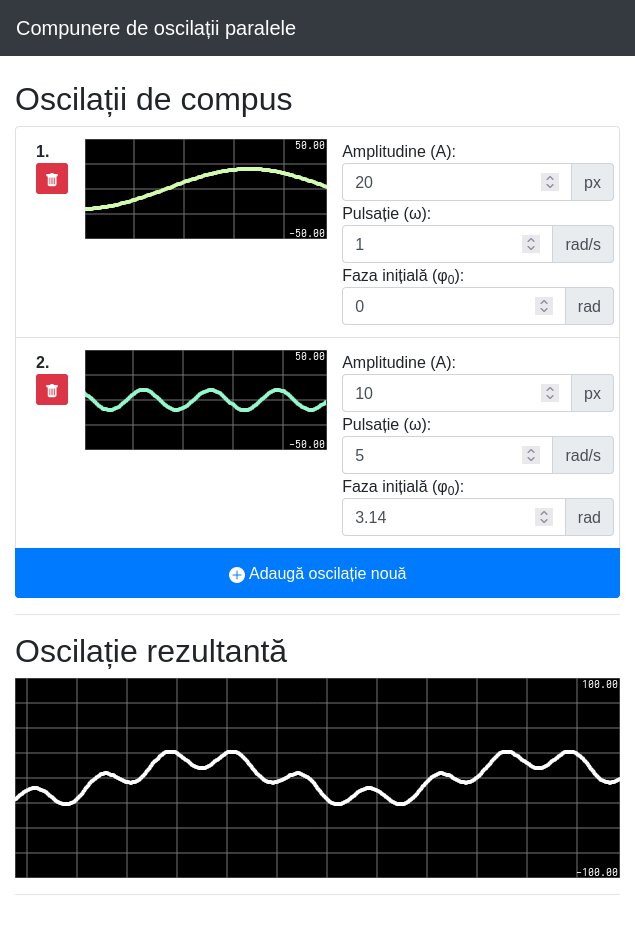
\includegraphics[width=0.4\linewidth]{biosc2}}
\end{figure}
Aplicația este alcătuită dintr-o singură pagină, ce conține titlul aplicației și interfața prin intermediul căreia se pot adăuga, modifica, elimina oscilații de compus, cu vizualizări dinamice atât pentru acestea cât și pentru oscilația rezultantă. Designul este unul adaptiv, putând fi utilizată facil și pe telefoane, și pe calculatoare.
\chapter{Tehnologii, limbaje, biblioteci folosite}
\begin{itemize}
	\item \textbf{React}: un framework de JavaScript care face crearea de aplicații web interactive cum este aceasta mult mai ușoară.
	\item \textbf{create-react-app}: interfață de creare de aplicații React ce configură diverse aplicații ajutătoare procesului de dezvoltare, cum ar fi \textbf{webpack}, cu care este produs din codul sursă un bundle optimizat de HTML, CSS și JavaScript.
	\item \textbf{TypeScript}: un fel de JavaScript, dar cu tipuri statice (ca în C++), ce compilează în JavaScript. În acest caz, este prezentă extensia de limbaj \textbf{JSX}, specifică Reactului.
	\item \textbf{HTML}: pentru scheletul paginii aplicației web.
	\item \textbf{CSS}: permite ajustarea aspectului aplicației web.
	\item \textbf{Bootstrap} prin \textbf{react-bootstrap} și prin \textbf{react-icons}: conține componente grafice (butoane, containere, iconițe etc.) facil de utilizat în astfel de aplicații web.
	\item \textbf{Smoothie charts} prin \textbf{react-smoothie}: face randarea facilă a oscilațiilor posibilă.
	\item \textbf{worker-timers}: facilitează ca randarea să se desfășoare corect chiar și atunci când tabul în care este încărcată aplicația nu este selectat.
	\item \textbf{randomColor}: permite generarea de culori pastelate care să fie asociate fiecărei oscilații, pentru a se diferenția.
\end{itemize}
\chapter{Cod sursă}
Codul sursă poate fi accesat pe \url{https://github.com/ALEX11BR/fizoscomp}. Mai jos sunt extrase din codul sursă:

\begin{minted}[linenos,breaklines,frame=single, label=public/index.html]{text}
<!DOCTYPE html>
<html lang="en">
  <head>
    <meta charset="utf-8" />
    <meta name="viewport" content="width=device-width, initial-scale=1" />
    <link rel="icon" href="%PUBLIC_URL%/favicon.ico" />
    <link rel="stylesheet" href="https://maxcdn.bootstrapcdn.com/bootstrap/4.5.0/css/bootstrap.min.css" integrity="sha384-9aIt2nRpC12Uk9gS9baDl411NQApFmC26EwAOH8WgZl5MYYxFfc+NcPb1dKGj7Sk" crossorigin="anonymous" />
    <title>Compunere oscilații paralele</title>
  </head>
  <body>
    <noscript>Activează-ți javascriptul!</noscript>
    <div id="root"></div>
  </body>
</html>

\end{minted}
\begin{minted}[linenos,breaklines,frame=single, label=src/index.css]{text}
.addbutton {
    text-align: center;
}
.listgroup {
    width: 100%;
}
\end{minted}
\begin{minted}[linenos,breaklines,frame=single, label=src/Osci.ts]{text}
export interface Osci {
  color: string;
  amplitudine: number;
  pulsatie: number;
  fazaInitiala: number;
}

export function fnFromOsci(osci: Osci) {
    return (i: number) => osci.amplitudine*Math.sin(osci.fazaInitiala + osci.pulsatie*i*40/1000);
}
\end{minted}
\begin{minted}[linenos,breaklines,frame=single, label=src/App.tsx]{text}
import React, { useState } from 'react';
import { Container, ListGroup, Row, Col, Navbar } from 'react-bootstrap';
import { BsPlusCircleFill } from 'react-icons/bs';
import randomColor from 'randomcolor';

import { fnFromOsci, Osci } from './Osci';
import Graph from './Graph';
import Oscilatie from './Oscilatie';

function App() {
  const [ oscilatii, setOscilatii ] = useState<Osci[]>([])
  function addOsci() {
    setOscilatii([ ...oscilatii, {
      color: randomColor({luminosity: 'light'}),
      amplitudine: oscilatii[0] ? oscilatii[0].amplitudine : 10,
      pulsatie: oscilatii[0] ? oscilatii[0].pulsatie : 1,
      fazaInitiala: oscilatii[0] ? oscilatii[0].fazaInitiala : 0
    }]);
  };
  function deleteOsci(index: number) {
    setOscilatii([
      ...oscilatii.slice(0,index),
      ...oscilatii.slice(index+1)
    ]);
  };
  function composedFn(i: number) {
    var r = 0;
    for (var oscilatie of oscilatii) {
      r+=fnFromOsci(oscilatie)(i);
    }
    return r;
  };
  return (
    <>
      <Navbar bg="dark" variant="dark">
        <Navbar.Brand>Compunere de oscilații paralele</Navbar.Brand>
      </Navbar>
      <br />
      <Container fluid>
        <Row>
          <Col xs={12} lg={6}>
            <h2>Oscilații de compus</h2>
            <ListGroup className={"listgroup"}>
              {oscilatii.map((oscilatie, index) => {
                return (
                  <Oscilatie
                    key={index}
                    index={index}
                    osci={oscilatie}
                    onDelete={() => deleteOsci(index)}
                    onUpdate={(o: Osci) => setOscilatii([
                      ...oscilatii.slice(0,index),
                      o,
                      ...oscilatii.slice(index+1)
                    ])}
                  />
                );
              })}
              <ListGroup.Item className="addbutton" action active onClick={addOsci}><BsPlusCircleFill /> Adaugă oscilație nouă</ListGroup.Item>
            </ListGroup>
            <hr />
          </Col>
          <Col xs={12} lg={6}>
            <h2>Oscilație rezultantă</h2>
            <Graph fn={composedFn} height={200} color="#ffffff" />
            <hr />
          </Col>
        </Row>
      </Container>
    </>
  );
}

export default App;
\end{minted}
\chapter{Manual de utilizare}
Aplicația \textit{Compunere de oscilații paralele} funcționează pe toate calculatoarele, telefoanele și tabletele cu browsere relevante în ziua de astăzi (adică nu Internet Explorer). Mai jos aveți instrucțiuni de utilizare:
\begin{enumerate}
  \item \ifig{initialAdd}
  Inițial nu vor fi oscilații de compus. Pentru a începe, adăugați o oscilație dând clic pe butonul \textit{Adaugă oscilație nouă}.
  \item \ifig{primoscAdd}
  Puteți ajusta parametrii oscilației. Puteți introduce acolo numere (chiar și cu zecimale, cu separatorul de parte zecimală fiind punctul). Câmpul de vizualizare a unei oscilații individuale are $50\times 2$ pixeli (iar cel al oscilației rezultante are maxim $100\times 2$ pixeli; puteți vedea aceste valori în colțurile din dreapta ale câmpurilor de vizualizare a oscilațiilor), așa că nu aș recomanda să treceți mai mult de 50 în dreptul amplitudinii unei oscilații, asta ca să poată fi văzută în întregime. În plus, valorile mari ale pulsației ($>20$) pot strica vizualizarea acesteia. Nu uitați că la orice adăugare/modificare/ștergere de oscilații randarea tuturor va fi reluată de la zero.
  \item \ifig{primoscNew}
  Repetați pașii 1 și 2 pentru a adăuga câte oscilații doriți.
  \item \ifig{triosc}
  Pentru a șterge o oscilație, apăsați pe butonul roșu cu coș de gunoi de sub numărul oscilației de șters.
\end{enumerate}
\chapter{Posibilități de dezvoltare}
Eu unul sunt mulțumit de starea în care se află aplicația. Cu toate acestea, recunosc că mai există caracteristici ce pot fi adăugate în cadrul aplicației, cum ar fi:
\begin{itemize}
  \item O pagină de teoria compunerii oscilațiilor paralele.
  \item Posibilitatea de a afișa, alături de oscilația rezultantă, în același câmp de vizualizare, și oscilațiile componente.
  \item Asigurarea că culorile generate pentru fiecare oscilație chiar le diferențiază.
  \item Posibilitatea de a ajusta culorile oscilațiilor.
  \item Posibilitatea de a activa/dezactiva oscilații fără a le șterge.
\end{itemize}
\end{document}
